\chapter{Managing Processes}
\section{Understanding Jobs and Processes}
During boot several services start up that in turn launch several processes that run in the background. They can be viewed by the \verb|ps aux| command. Everything that's happening on a Linux system has a \textbf{process} behind it, which controls the actions. However, sometimes users launch a process from the shell - then it's called a \textbf{job}, related to that specific shell. 

Let us consider a situation where a job keeps a shell busy. Consider the command is :

\vspace{-15pt}
\begin{minted}{console}
# dd if=/dev/zero of=/dev/null # Copies Nothing to Nowhere!
\end{minted}
\vspace{-10pt}

To stop the job from keeping the shell busy, we can move it to the background. The first step is to stop the job using \textit{CTRL+Z}. Then, simply typing bg moves the job to the background!

\subsection{jobs}
The jobs command shows us an overview of all the jobs that are currently running. 

\vspace{-15pt}
\begin{minted}{console}
$ dd if=/dev/zero of=/dev/null
^Z
[1]+  Stopped                 dd if=/dev/zero of=/dev/null
$ jobs
[1]+  Stopped                 dd if=/dev/zero of=/dev/null
$ bg
[1]+ dd if=/dev/zero of=/dev/null &
$ jobs
[1]+  Running                 dd if=/dev/zero of=/dev/null &
\end{minted}
\vspace{-10pt}

\noindent
Jobs are tied to the current shell and user account. Any user will only see the jobs that were launched using the present shell when the \verb|jobs| command is used.

	\section{Managing Shell Jobs} 
Every command on the shell is considered a shell job. Many of them start and stop immediately (execute very fast) because they've completed their task. 

\vspace{-15pt}
\begin{minted}{console}
$ ls
Desktop    Downloads  Pictures  Public     Videos
Documents  Music      Programs  Templates
\end{minted}
\vspace{-10pt}

\noindent
Other programs may need us to wait while they finish their jobs. In such cases, we can put them to work in the background and not have them obstruct our work. 

\vspace{-15pt}
\begin{minted}{console}
$ cat test.sh
#!/bin/bash
echo "Starting"
sleep 10
echo "Completed!"
$ ./test.sh
Starting
^Z
[1]+  Stopped                 ./test.sh
$ jobs
[1]+  Stopped                 ./test.sh
$ bg
[1]+ ./test.sh &
$ Completed!

[1]+  Done                    ./test.sh
$ ./test.sh &
[1] 39773
Starting
$ Completed!

[1]+  Done                    ./test.sh
\end{minted}
\vspace{-10pt}

\noindent
To directly start a job in the background, we need only suffix the command with a \verb|&|. If we have multiple commands running in the background, we can put any one of them in the foreground using: \verb|fg <jobId>|. Similarly, to kill a job, simply type: \verb|%<jobId>|.

\vspace{-15pt}
\begin{minted}{console}
$ sleep 600 &
[1] 41461
$ dd if=/dev/zero of=/dev/null
^Z
[2]+  Stopped                 dd if=/dev/zero of=/dev/null
$ jobs
[1]-  Running                 sleep 600 &
[2]+  Stopped                 dd if=/dev/zero of=/dev/null
$ bg 
[2]+ dd if=/dev/zero of=/dev/null &
$ jobs
[1]-  Running                 sleep 600 &
[2]+  Running                 dd if=/dev/zero of=/dev/null &
$ fg 1
sleep 600
^C
$ fg
dd if=/dev/zero of=/dev/null
^Z
[2]+  Stopped                 dd if=/dev/zero of=/dev/null
$ jobs
[2]+  Stopped                 dd if=/dev/zero of=/dev/null
$ kill %2
[2]+  Terminated              dd if=/dev/zero of=/dev/null
$ jobs
$ 
\end{minted}
\vspace{-10pt}

	\section{Getting process information with ps}
\begin{itemize}
	\item Shows a snapshot of all the running processes.
	\item \verb|ps| shows only user's own processes. 
	
	\item \verb|ps aux| shows the processes of all users with the following details:
	
	\begin{tabular}{cM{0.75}}
		\toprule
		\textbf{Option} &\textbf{Description} \\
		\midrule
		\textbf{a} &Show processes for all users \\
		\textbf{u} &Display the process's user/owner \\
		\textbf{x} &Also show processes not attached to a terminal \\
		\bottomrule
	\end{tabular}
	
	\noindent
	To see only the first 10 processes, use:
	\vspace{-15pt}
	\begin{minted}{console}
	# ps aux | head
	USER        PID %CPU %MEM    VSZ   RSS TTY      STAT START   TIME COMMAND
	root          1  0.0  0.3 128164  6852 ?        Ss   Nov28   0:16 /usr/lib/systemd/systemd --switched-root --system --deserialize 21
	root          2  0.0  0.0      0     0 ?        S    Nov28   0:00 [kthreadd]
	root          3  0.0  0.0      0     0 ?        S    Nov28   0:09 [ksoftirqd/0]
	root          5  0.0  0.0      0     0 ?        S<   Nov28   0:00 [kworker/0:0H]
	root          7  0.0  0.0      0     0 ?        S    Nov28   0:00 [migration/0]
	root          8  0.0  0.0      0     0 ?        S    Nov28   0:00 [rcu_bh]
	root          9  0.0  0.0      0     0 ?        R    Nov28   0:42 [rcu_sched]
	root         10  0.0  0.0      0     0 ?        S    Nov28   0:02 [watchdog/0]
	root         12  0.0  0.0      0     0 ?        S    Nov28   0:00 [kdevtmpfs]
	\end{minted}
	\vspace{-10pt}
	
	\begin{itemize}
		\item The \textbf{PID} is the Process ID assigned to each process automatically by the Kernel. The PID 1 process is Systemd, which is the first process started by the kernel, which in turn starts all other processes.
		
		\item \textbf{\%CPU} and \textbf{\%MEM} are the CPU and Memory usage stats. \textit{VSZ} is the Virtual Memory (total memory that the process has access to) while Resident Set Size (\textit{RSS}) refers to the Physical Memory being used by the process. \textit{Note that this includes the dynamic libraries, so if a library is used by a module multiple times, the memory used by the process will be smaller than the RSS}.
		
		\item \textbf{TTY} represents the terminal number on which the process is running. For background process, the TTY will be shown as \verb|?|. 
		
		\item \textbf{STAT} is the status of the process. \textit{S} indicates the process is asleep. 
		
		\item \textbf{TIME} is the total runtime of the process.
		\item \textbf{COMMAND} is the command that was executed.
	\end{itemize}
\end{itemize}

Normally, we use \verb|ps aux| to get the PID of a process. We can see the terminal grep itself is running on is set to \verb|pts/0|, which is the gnome terminal. 

\subsection{Getting PID of a process}
To see the PID of a particular process we simply grep some keyword related to the process, typically the process name. 

\vspace{-15pt}
\begin{minted}{console}
# ps aux | grep packagekitd
root       1680  0.0  0.3 480016  5752 ?        Ssl  Nov28   0:05 /usr/libexec/packagekitd
root      44081  0.0  0.0 112660   976 pts/0    R+   21:04   0:00 grep --color=auto packagekitd
\end{minted}
\vspace{-10pt}

The \verb|R| status indicates that the command \verb|grep| was running at the time.

\subsubsection{w command}
\vspace{-10pt}
The \verb|w| command shows all the logged in users, what they're doing and the consequent load on the system. 

\vspace{-15pt}
\begin{minted}{console}
# w
20:58:00 up 2 days,  1:09,  2 users,  load average: 0.00, 0.01, 0.05
USER     TTY      FROM             LOGIN@   IDLE   JCPU   PCPU WHAT
somu     :0       :0               Mon09   ?xdm?   1:12m  0.84s /usr/libexec/gnome-session-binary --session gnome-classic
somu     pts/0    :0               13:41    0.00s  0.67s 10.88s /usr/libexec/gnome-terminal-server
\end{minted}
\vspace{-10pt}

\subsection{Seeing Parent and Child process relation}
Sometimes we need to see the relation between the processes, because when we kill a parent process, the child processes are also killed automatically! For that we use the command \verb|ps fax|. 

\vspace{-15pt}
\begin{minted}{console}
# ps fax | tail
37204 ?        S      0:00  \_ gnome-pty-helper
37205 pts/0    Ss     0:00  \_ bash
43222 pts/0    S      0:00      \_ su -
43230 pts/0    S      0:00          \_ -bash
43291 pts/0    S      0:00              \_ su - somu
43292 pts/0    S      0:00                  \_ -bash
43465 pts/0    S      0:00                      \_ su
43471 pts/0    S      0:00                          \_ bash
44146 pts/0    R+     0:00                              \_ ps fax
44147 pts/0    D+     0:00                              \_ [tail]
\end{minted}
\vspace{-10pt}

	\section{Understanding Memory Usage}
To get an overview of the free memory available we use the command \verb|free -m| where \verb|-m| stands for Mega-Bytes. \textit{Free} is the unused physical RAM. \textit{Shared} refers to the memory used by shared libraries (shared by different programs). \textit{buff/cache} is the combined Buffer and/or cache usage, where buffer is typically used when there's a large amount of data that needs to be committed to disk. \textit{Available} is the amount of memory available for starting new applications without swapping. 

\vspace{-15pt}
\begin{minted}{console}
# free -m
total        used        free      shared  buff/cache   available
Mem:           1823         930         198          18         694         656
Swap:          1907           0        1907
\end{minted}
\vspace{-10pt}

\textbf{Swap} contains the unused memory pages from the RAM that have been transfered to the Hard disk. 

	\section{Understanding Performance Load}
When a process is ready for execution, it's added to the runqueue, where it awaits evaluation by the scheduler to be assigned to a CPU. The amount of processes awaiting to be executed determines the performance load. 

\begin{figure}[H]
	\centering
	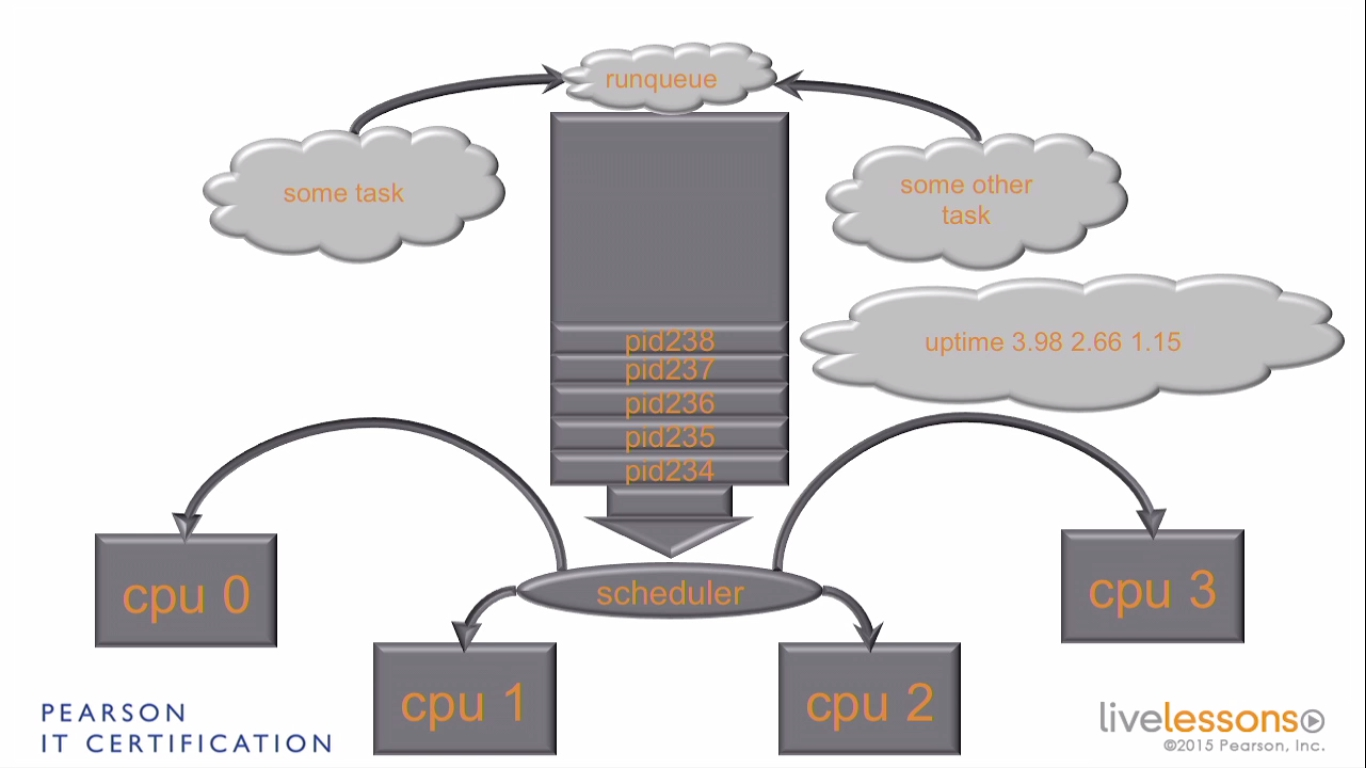
\includegraphics[width=0.9\linewidth]{Mod2/chapters/2.10.a}
	\caption{Performance Load}
	\label{fig:2}
\end{figure}

\subsection{uptime Command}
The \verb|uptime| command shows us how long the system has been on, the number of users logged on and a snapshot of the current CPU demand for the last 1, 5 and 15 minutes, in that order. However, this number is represented for the total CPU resources being used, and not an average! Thus, for a single CPU system, uptime of 1 = 100\% usage, while for a 4 CPU system, it means the CPU has been 75\% idle. 

The \textit{System Load Average} is the number of processes in the runqueue that are either in runnable (ready to run/already running) state or in an interruptible state (e.g., waiting for I/O access). 

\vspace{-15pt}
\begin{minted}{console}
# uptime
11:59:13 up 2 days,  6:02,  2 users,  load average: 0.00, 0.01, 0.05
\end{minted}
\vspace{-10pt}

\noindent
The \verb|nproc| command shows us the number of CPU cores available to us. 

\vspace{-15pt}
\begin{minted}{console}
# nproc
1
\end{minted}
\vspace{-10pt}

	\section{Monitoring System Activity with top}
\textbf{top} shows us the top active processes on the system in real-time. 

\vspace{-15pt}
\begin{minted}{console}
# top
top - 12:24:09 up 2 days,  6:27,  2 users,  load average: 0.15, 0.07, 0.06
Tasks: 207 total,   2 running, 205 sleeping,   0 stopped,   0 zombie
%Cpu(s):  3.9 us,  0.7 sy,  0.0 ni, 95.4 id,  0.0 wa,  0.0 hi,  0.0 si,  0.0 st
KiB Mem :  1867024 total,   196468 free,   957244 used,   713312 buff/cache
KiB Swap:  1953788 total,  1953788 free,        0 used.   667488 avail Mem 

PID USER      PR  NI    VIRT    RES    SHR S %CPU %MEM     TIME+ COMMAND                                                                    
2023 somu      20   0 1943348 246224  49292 S  5.3 13.2  61:53.62 gnome-shell                                                                
2250 somu      20   0  525584  12240   5984 S  2.3  0.7   0:00.61 tracker-store                                                              
1367 root      20   0  291800  35340  10312 S  1.3  1.9   2:53.91 X                                                                          
48709 root      20   0  157716   2284   1536 R  0.7  0.1   0:00.06 top                                                                        
764 root      20   0  305080   6140   4768 R  0.3  0.3   6:45.26 vmtoolsd                                                                   
2270 somu      20   0  385944  19688  15236 S  0.3  1.1   6:02.21 vmtoolsd                                                                   
2290 somu      39  19  637720  11280   8036 S  0.3  0.6   0:00.52 tracker-miner-f                                                            
48449 root      20   0       0      0      0 S  0.3  0.0   0:00.80 kworker/0:0                                                                
1 root      20   0  128164   6852   4084 S  0.0  0.4   0:18.42 systemd                                                                    
2 root      20   0       0      0      0 S  0.0  0.0   0:00.22 kthreadd                                                                   
3 root      20   0       0      0      0 S  0.0  0.0   0:11.45 ksoftirqd/0                                                                
5 root       0 -20       0      0      0 S  0.0  0.0   0:00.00 kworker/0:0H                                                               
7 root      rt   0       0      0      0 S  0.0  0.0   0:00.00 migration/0                                                                
8 root      20   0       0      0      0 S  0.0  0.0   0:00.00 rcu_bh                                                                     
9 root      20   0       0      0      0 S  0.0  0.0   0:48.31 rcu_sched                                                                  
10 root      rt   0       0      0      0 S  0.0  0.0   0:02.52 watchdog/0                                                                 
12 root      20   0       0      0      0 S  0.0  0.0   0:00.00 kdevtmpfs                                                                  
13 root       0 -20       0      0      0 S  0.0  0.0   0:00.00 netns                                                                      
14 root      20   0       0      0      0 S  0.0  0.0   0:00.22 khungtaskd                                                                 
15 root       0 -20       0      0      0 S  0.0  0.0   0:00.00 writeback                                                                  
16 root       0 -20       0      0      0 S  0.0  0.0   0:00.00 kintegrityd                                                                
17 root       0 -20       0      0      0 S  0.0  0.0   0:00.00 bioset                                                                     
18 root       0 -20       0      0      0 S  0.0  0.0   0:00.00 kblockd                                                                    
19 root       0 -20       0      0      0 S  0.0  0.0   0:00.00 md                                                                         
25 root      20   0       0      0      0 S  0.0  0.0   0:00.20 kswapd0                                                                    
\end{minted}
\vspace{-10pt}

\noindent
If we put 3 processes that all run \verb|dd if=/dev/zero of=/dev/null| on the runqueue, and then execute the \verb|top| command, and then press the \verb|1| key, all the individual CPU loads are displayed. Since our VM has only one CPU, it shows up as \textit{Cpu0}.

\vspace{-15pt}
\begin{minted}{console}
# top
...
%Cpu0  : 27.6 us, 72.4 sy,  0.0 ni,  0.0 id,  0.0 wa,  0.0 hi,  0.0 si,  0.0 st
...
PID USER      PR  NI    VIRT    RES    SHR S %CPU %MEM     TIME+ COMMAND                                                                    
48739 root      20   0  107948    612    516 R 32.9  0.0   0:04.59 dd                                                                         
48737 root      20   0  107948    612    516 R 32.2  0.0   0:06.47 dd                                                                         
48738 root      20   0  107948    608    516 R 32.2  0.0   0:04.94 dd                                                                         
\end{minted}
\vspace{-10pt}

\noindent
The first line of the output of the \verb|top| command is the same as that of the \verb|uptime| command. The top command also shows the Free and available memory in both physical RAM as well as Swap. 

Now since there is only one cpu available, the 3 busiest processes, (the \verb|dd| commands) have evenly distributed the CPU cycles among them (assigned by the scheduler), nearly 33\% each (the rest is overheads and cycles used by other processes).

\noindent
\verb|%Cpu(s): 26.5 us, 73.5 sy,  0.0 ni,  0.0 id,  0.0 wa,  0.0 hi,  0.0 si,  0.0 st| 

The CPU line shows the CPU Usage stats in percentages. Here, we see the CPU usage summary [Cpu(s)], the \textit{us} stands for user-space, or processes started by the user. The \textit{sy}  shows us the system space CPU Usage, and is typically programs that directly deal with hardware. Since we've used the \verb|dd| command that's directly copying data from one device to another, we have a high system space CPU usage. 

The \textit{id} stands for idle and shows us the percentage of time the system is idle. The \textit{wa} shows the percentage of time the system is waiting for I/O operation completion, such as a slow disk or network. 

	\section{Sending Signals to processes}
Signals are mandatory instructions that the process can't ignore. Some of the most common Signals are \textbf{SIGTERM} and \textbf{SIGKILL}. The \verb|SIGTERM| signal asks a process to cease its activity. If the signal doesn't work, i.e., the process doesn't obey it, then we send the \verb|SIGKILL| signal, which terminates the process. 

We can send these signals by the use of the \verb|top| command. While top is running, we have to press the \verb|k| key to initiate signal sending via \verb|kill|. To choose the appropriate process, we enter the PID. The default signal is \verb|SIGTERM| (a.k.a. Signal 15). The process is terminated immediately on sending the signal. 

When we send Signal 9 (\verb|SIGKILL|) the process doesn't have time to save or clean up its work, and thus the execution stops instantaneously! This means if a process is working on an open file, the \verb|SIGKILL| signal can cause irreparable damage to it. 

\subsection{kill command}
To send a signal directly from the command line, we use the \verb|kill| command. To send a \verb|SIGTERM| signal, we merely provide the PID. To send a \verb|SIGKILL| signal, we have to provide a signal number of \verb|9|. 

\vspace{-15pt}
\begin{minted}{console}
# ps aux | grep dd
...
root      49575 50.3  0.0 107948   608 pts/0    R    13:25   
[2]+  Running                 dd if=/dev/zero of=/dev/null &
# kill -9 49575
# jobs
[2]+  Killed                  dd if=/dev/zero of=/dev/null
\end{minted}
\vspace{-10pt}

To kill all processes matching a certain process using Signals uses:

\vspace{-15pt}
\begin{minted}{console}
# top
...
PID USER      PR  NI    VIRT    RES    SHR S %CPU %MEM     TIME+ COMMAND                                                                    
49747 root      20   0  107948    608    516 R 22.8  0.0   0:05.81 dd                                                                         
49748 root      20   0  107948    612    516 R 22.5  0.0   0:05.30 dd                                                                         
49749 root      20   0  107948    612    516 R 22.5  0.0   0:04.91 dd                                                                         
49746 root      20   0  107948    612    516 R 22.2  0.0   0:06.60 dd                                                                         
...
# jobs
[1]   Running                 dd if=/dev/zero of=/dev/null \&
[2]   Running                 dd if=/dev/zero of=/dev/null \&
[3]-  Running                 dd if=/dev/zero of=/dev/null \&
[4]+  Running                 dd if=/dev/zero of=/dev/null \&
# killall dd
# jobs
[1]   Terminated              dd if=/dev/zero of=/dev/null
[2]   Terminated              dd if=/dev/zero of=/dev/null
[3]-  Terminated              dd if=/dev/zero of=/dev/null
[4]+  Terminated              dd if=/dev/zero of=/dev/null
\end{minted}
\vspace{-10pt}

	\section{Understanding Priorities and Niceness}
Consider a hypothetical scenario where a bunch of people are standing in a queue to get movie tickets. There, everyone in the queue has the same priority. Now, if a lady comes along and skips the queue, we can fairly say she isn't nice. The same goes for processes in a Linux system.

The processes are born with the same priority, but their niceness can be adjusted. If the niceness is negative, the process is served first, and if positive, it lets the other processes (with lower niceness) be served before itself!

\section{Changing Process Nice values}
In the output of the \verb|top| command, the \textit{PR} column shows us the priority of each individual process. Normal processes are started with the same priority of \textbf{20}. There are certain real-time processes as well, that have a value of \verb|rt| in their priority column.

In case we need to increase or decrease the priority of a process (e.g., higher priority to quickly complete a query, or free resources for other users by lowering priority) we adjust the niceness (\textit{NI}) value of the process. This process is called \textit{nicing} a process. 

The niceness of a process can range from $-20$ to $+19$, and the consequent value of priority is related as : $$PR = 20 + NI$$ Thus, the priority of a process can range from $0$ (most aggressive) to $39$ (nicest). We can adjust the niceness in small increments instead of huge jumps (setting niceness to $-20$) and see if that does our work. If not, we can change the niceness incrementally till our goals are met!

\subsection{Chaning niceness from top}
To renice a process from top, we can simply press \verb|r|, then select the PID to renice and enter the new niceness value.

\subsection{Changing Niceness from command line}
We can also set the niceness from the command line, both while first running the process using the \verb|nice| command, or change the nice value of a running process using the \verb|renice| command. 

\vspace{-15pt}
\begin{minted}{console}
# nice -n 10 dd if=/dev/zero of=/dev/null &
# top | head
top - 15:40:26 up 2 days,  9:44,  3 users,  load average: 1.10, 0.70, 0.71
Tasks: 215 total,   3 running, 212 sleeping,   0 stopped,   0 zombie
%Cpu(s):  9.5 us, 71.4 sy, 19.0 ni,  0.0 id,  0.0 wa,  0.0 hi,  0.0 si,  0.0 st
KiB Mem :  1867024 total,   233356 free,   919716 used,   713952 buff/cache
KiB Swap:  1953788 total,  1953788 free,        0 used.   704744 avail Mem 

PID USER      PR  NI    VIRT    RES    SHR S %CPU %MEM     TIME+ COMMAND                                                                    
51465 root      30  10  107948    612    516 R 75.0  0.0   2:00.96 dd                                                                         
1367 root      20   0  290560  34108  10412 S  5.0  1.8   3:22.26 X                                                                          
2023 somu      20   0 1923992 226836  49300 S  5.0 12.1  66:10.12 gnome-shell                                                                
# renice -n -10 51465
51465 (process ID) old priority 10, new priority -10
# top | head
top - 15:42:18 up 2 days,  9:45,  3 users,  load average: 1.41, 0.92, 0.79
Tasks: 215 total,   2 running, 213 sleeping,   0 stopped,   0 zombie
%Cpu(s): 25.0 us, 75.0 sy,  0.0 ni,  0.0 id,  0.0 wa,  0.0 hi,  0.0 si,  0.0 st
KiB Mem :  1867024 total,   233440 free,   919632 used,   713952 buff/cache
KiB Swap:  1953788 total,  1953788 free,        0 used.   704828 avail Mem 

PID USER      PR  NI    VIRT    RES    SHR S %CPU %MEM     TIME+ COMMAND                                                                    
51465 root      10 -10  107948    612    516 R 64.0  0.0   3:47.16 dd                                                                         
1 root      20   0  128164   6852   4084 S  0.0  0.4   0:19.34 systemd                                                                    
2 root      20   0       0      0      0 S  0.0  0.0   0:00.23 kthreadd                                    
\end{minted}
\vspace{-10pt}

\noindent
If however we find that we have to renice processes all the time, we might want to move some resource-hungry processes to other server(s). 

